% Editable textbook TikZ, initially imported from the verified semantic plate.
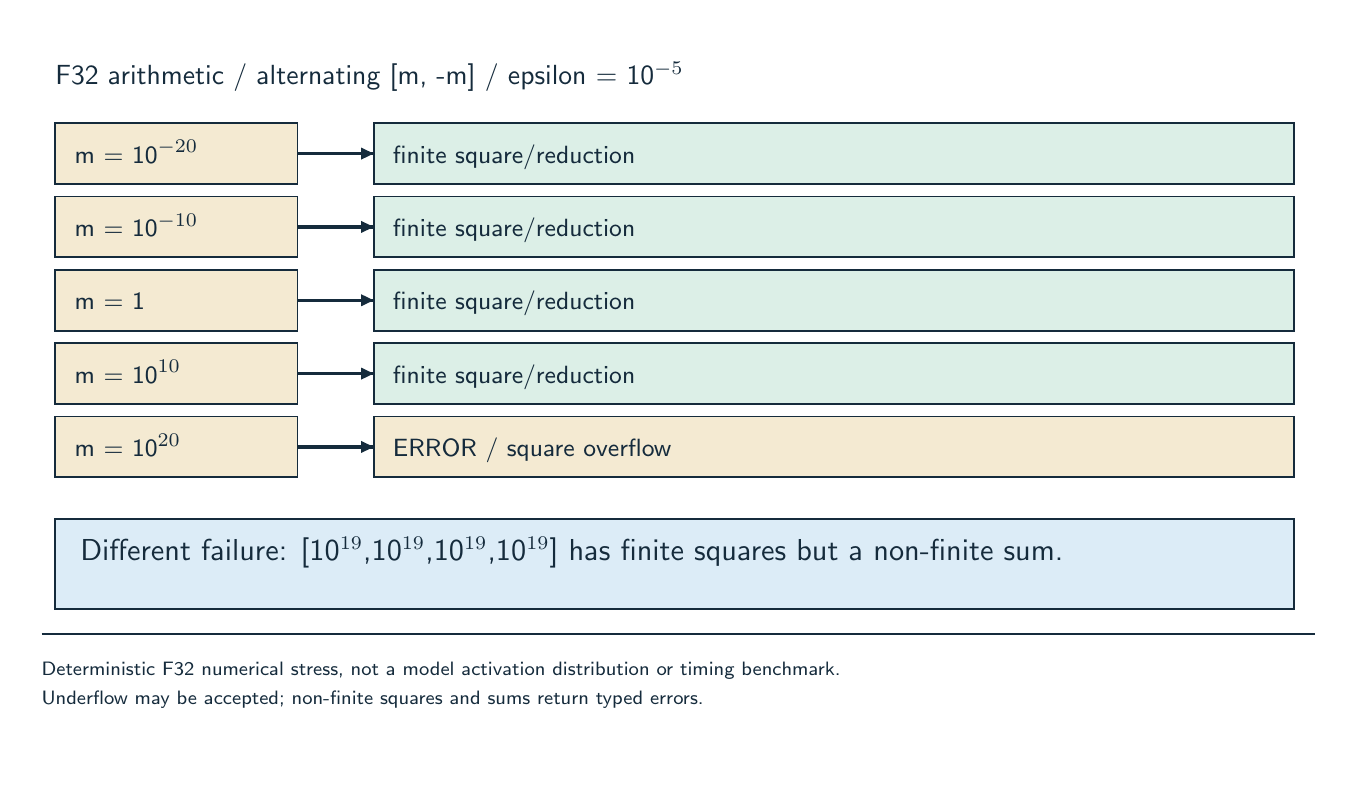
\begin{tikzpicture}[x=.5pt,y=-.5pt]
\path[use as bounding box] (30,170) rectangle (975,700);
\node[inner sep=0pt,outer sep=0pt,anchor=base west,text={rgb,255:red,21;green,43;blue,60},font=\sffamily\fontsize{10.0}{12.0}\selectfont] at (50,211) {F32 arithmetic / alternating [m, -m] / epsilon = 10\({}^{-5}\)};
\path[fill={rgb,255:red,244;green,234;blue,210},draw={rgb,255:red,21;green,43;blue,60},line width=0.7pt] (50.0,239.0) rectangle (225.0,283.0);
\node[inner sep=0pt,outer sep=0pt,anchor=base west,text={rgb,255:red,21;green,43;blue,60},font=\sffamily\fontsize{9.5}{11.4}\selectfont] at (64,268) {m = 10\({}^{-20}\)};
\draw[fill=none,draw={rgb,255:red,21;green,43;blue,60},line width=1.25pt] (225,261) -- (280,261);
\path[fill={rgb,255:red,21;green,43;blue,60},draw=none,line width=0.5pt] (280.00,261.00) -- (271.00,265.35) -- (271.00,256.65) -- cycle;
\path[fill={rgb,255:red,220;green,239;blue,231},draw={rgb,255:red,21;green,43;blue,60},line width=0.7pt] (280.0,239.0) rectangle (945.0,283.0);
\node[inner sep=0pt,outer sep=0pt,anchor=base west,text={rgb,255:red,21;green,43;blue,60},font=\sffamily\fontsize{9.5}{11.4}\selectfont] at (294,268) {finite square/reduction};
\path[fill={rgb,255:red,244;green,234;blue,210},draw={rgb,255:red,21;green,43;blue,60},line width=0.7pt] (50.0,292.0) rectangle (225.0,336.0);
\node[inner sep=0pt,outer sep=0pt,anchor=base west,text={rgb,255:red,21;green,43;blue,60},font=\sffamily\fontsize{9.5}{11.4}\selectfont] at (64,321) {m = 10\({}^{-10}\)};
\draw[fill=none,draw={rgb,255:red,21;green,43;blue,60},line width=1.25pt] (225,314) -- (280,314);
\path[fill={rgb,255:red,21;green,43;blue,60},draw=none,line width=0.5pt] (280.00,314.00) -- (271.00,318.35) -- (271.00,309.65) -- cycle;
\path[fill={rgb,255:red,220;green,239;blue,231},draw={rgb,255:red,21;green,43;blue,60},line width=0.7pt] (280.0,292.0) rectangle (945.0,336.0);
\node[inner sep=0pt,outer sep=0pt,anchor=base west,text={rgb,255:red,21;green,43;blue,60},font=\sffamily\fontsize{9.5}{11.4}\selectfont] at (294,321) {finite square/reduction};
\path[fill={rgb,255:red,244;green,234;blue,210},draw={rgb,255:red,21;green,43;blue,60},line width=0.7pt] (50.0,345.0) rectangle (225.0,389.0);
\node[inner sep=0pt,outer sep=0pt,anchor=base west,text={rgb,255:red,21;green,43;blue,60},font=\sffamily\fontsize{9.5}{11.4}\selectfont] at (64,374) {m = 1};
\draw[fill=none,draw={rgb,255:red,21;green,43;blue,60},line width=1.25pt] (225,367) -- (280,367);
\path[fill={rgb,255:red,21;green,43;blue,60},draw=none,line width=0.5pt] (280.00,367.00) -- (271.00,371.35) -- (271.00,362.65) -- cycle;
\path[fill={rgb,255:red,220;green,239;blue,231},draw={rgb,255:red,21;green,43;blue,60},line width=0.7pt] (280.0,345.0) rectangle (945.0,389.0);
\node[inner sep=0pt,outer sep=0pt,anchor=base west,text={rgb,255:red,21;green,43;blue,60},font=\sffamily\fontsize{9.5}{11.4}\selectfont] at (294,374) {finite square/reduction};
\path[fill={rgb,255:red,244;green,234;blue,210},draw={rgb,255:red,21;green,43;blue,60},line width=0.7pt] (50.0,398.0) rectangle (225.0,442.0);
\node[inner sep=0pt,outer sep=0pt,anchor=base west,text={rgb,255:red,21;green,43;blue,60},font=\sffamily\fontsize{9.5}{11.4}\selectfont] at (64,427) {m = 10\({}^{10}\)};
\draw[fill=none,draw={rgb,255:red,21;green,43;blue,60},line width=1.25pt] (225,420) -- (280,420);
\path[fill={rgb,255:red,21;green,43;blue,60},draw=none,line width=0.5pt] (280.00,420.00) -- (271.00,424.35) -- (271.00,415.65) -- cycle;
\path[fill={rgb,255:red,220;green,239;blue,231},draw={rgb,255:red,21;green,43;blue,60},line width=0.7pt] (280.0,398.0) rectangle (945.0,442.0);
\node[inner sep=0pt,outer sep=0pt,anchor=base west,text={rgb,255:red,21;green,43;blue,60},font=\sffamily\fontsize{9.5}{11.4}\selectfont] at (294,427) {finite square/reduction};
\path[fill={rgb,255:red,244;green,234;blue,210},draw={rgb,255:red,21;green,43;blue,60},line width=0.7pt] (50.0,451.0) rectangle (225.0,495.0);
\node[inner sep=0pt,outer sep=0pt,anchor=base west,text={rgb,255:red,21;green,43;blue,60},font=\sffamily\fontsize{9.5}{11.4}\selectfont] at (64,480) {m = 10\({}^{20}\)};
\draw[fill=none,draw={rgb,255:red,21;green,43;blue,60},line width=1.25pt] (225,473) -- (280,473);
\path[fill={rgb,255:red,21;green,43;blue,60},draw=none,line width=0.5pt] (280.00,473.00) -- (271.00,477.35) -- (271.00,468.65) -- cycle;
\path[fill={rgb,255:red,244;green,234;blue,210},draw={rgb,255:red,21;green,43;blue,60},line width=0.7pt] (280.0,451.0) rectangle (945.0,495.0);
\node[inner sep=0pt,outer sep=0pt,anchor=base west,text={rgb,255:red,21;green,43;blue,60},font=\sffamily\fontsize{9.5}{11.4}\selectfont] at (294,480) {ERROR / square overflow};
\path[fill={rgb,255:red,220;green,236;blue,247},draw={rgb,255:red,21;green,43;blue,60},line width=0.7pt] (50.0,525.0) rectangle (945.0,590.0);
\node[inner sep=0pt,outer sep=0pt,anchor=base west,text={rgb,255:red,21;green,43;blue,60},font=\sffamily\fontsize{9.5}{11.4}\selectfont] at (64,554) {};
\node[inner sep=0pt,outer sep=0pt,anchor=base west,text={rgb,255:red,21;green,43;blue,60},font=\sffamily\fontsize{10.5}{12.6}\selectfont] at (68,555) {Different failure: [10\({}^{19}\),10\({}^{19}\),10\({}^{19}\),10\({}^{19}\)] has finite squares but a non-finite sum.};
\draw[fill=none,draw={rgb,255:red,21;green,43;blue,60},line width=0.75pt] (40,608) -- (960,608);
\node[inner sep=0pt,outer sep=0pt,anchor=base west,text={rgb,255:red,21;green,43;blue,60},font=\sffamily\fontsize{7.5}{9.0}\selectfont] at (40,638) {Deterministic F32 numerical stress, not a model activation distribution or timing benchmark.};
\node[inner sep=0pt,outer sep=0pt,anchor=base west,text={rgb,255:red,21;green,43;blue,60},font=\sffamily\fontsize{7.5}{9.0}\selectfont] at (40,659) {Underflow may be accepted; non-finite squares and sums return typed errors.};
\end{tikzpicture}
